\begin{refsection}

\chapter{U--Pb}
\label{ch:UPb-R}

\noindent\begin{minipage}[t]{.5\linewidth}
\strut\vspace*{-\baselineskip}\newline
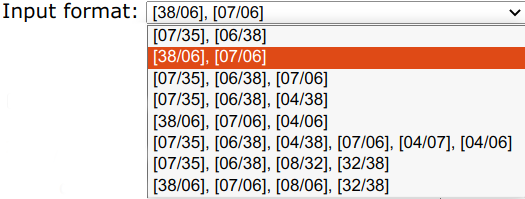
\includegraphics[width=\linewidth]{../figures/UPbFormats.png}\\
\end{minipage}
\begin{minipage}[t]{.5\textwidth}
  \texttt{IsoplotR} accommodates eight U--Pb formats. See
  Section~\ref{sec:UPbFormats} for details.
\end{minipage}

\noindent Examples using the CLI:

\begin{script}
# U-Pb format 1, 1se absolute input errors:
UPb1 <- read.data('UPb1.csv',method='U-Pb',format=1)
# U-Pb format 6, 1se relative input errors:
UPb2 <- read.data('UPb6.csv',method='U-Pb',format=6,ierr=3)
# U-Pb format 8, 2se relative input errors:
UPb3 <- read.data('UPb8.csv',method='U-Pb',format=8,ierr=4)
\end{script}

\noindent where \texttt{UPb1.csv}, \texttt{UPb6.csv} and
\texttt{UPb8.csv} are files that are included in \texttt{IsoplotR} and
whose file path can be found as follows:

\begin{console}
fn <- system.file('UPb1.csv',package='IsoplotR')
\end{console}

\noindent\begin{minipage}[t]{.15\linewidth}
\strut\vspace*{-\baselineskip}\newline
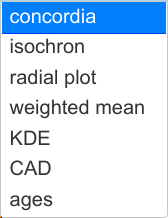
\includegraphics[width=\linewidth]{../figures/UPbPlotdevices.png}
\end{minipage}
\begin{minipage}[t]{.85\textwidth}
  U--Pb data can be visualised on five or six different plot devices
  and output tables. The \texttt{isochron} option is only available
  for formats 4--8 and is invisible otherwise. See the remaining
  sections of this chapter for examples of these output options.
\end{minipage}

\section{General options}
\label{sec:general}

\begin{enumerate}

  \item\label{it:UPbLambdairatio} Isotopic ratios and decay constants:

\noindent\begin{minipage}[t]{.55\linewidth}
\strut\vspace*{-\baselineskip}\newline
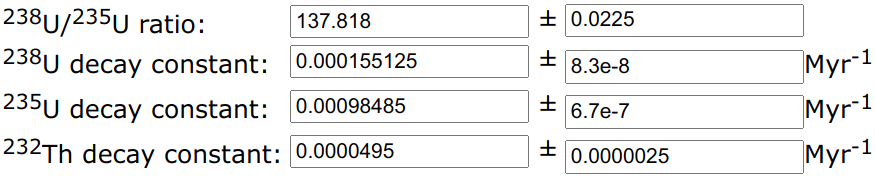
\includegraphics[width=\linewidth]{../figures/UPbLambda.png}
\end{minipage}
\begin{minipage}[t]{.45\linewidth}
  The default \textsuperscript{238}U/\textsuperscript{235}U ratio is
  given by \citet{hiess2012}, and the U and Th decay constants by
  \citet{jaffey1971} and \citet{leroux1963}, respectively. These
  values and their uncertainties can be changed here.
\end{minipage}

\begin{script}
# use the Steiger and Jaeger (1977) value with zero uncertainty
settings('iratio','U238U235',137.88,0)
# use the Schoene et al. (2006) value and uncertainty
settings('lambda','U238',0.000154993,0.00000013) 
\end{script}

\item Common Pb correction of the individual aliquots can be carried
  out using the methods of Section~\ref{sec:common-Pb}. This may be
  useful for single grain analysis tools such as the KDE, CAD, radial
  or weighted mean plot. For cogenetic aliquots that form an isochron,
  the common Pb is best left uncorrected. In this case the most
  reliable age estimate is given by the isochron through the
  uncorrected data, which can be visualised on a concordia diagram
  (Section~\ref{sec:concordia-R}) or (for formats 4--8) as a separate
  isochron plot (Section~\ref{sec:UPb-isochron-R}).

\noindent\begin{minipage}[t]{.4\linewidth}
\strut\vspace*{-\baselineskip}\newline
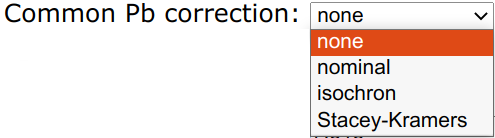
\includegraphics[width=\linewidth]{../figures/CommonPb.png}
\end{minipage}
\begin{minipage}[t]{.6\linewidth}
  A common Pb menu is available for all output types except
  \texttt{isochron}. It gives access to four different common Pb
  treatments that can be applied to the data before plotting.
\end{minipage}

\begin{enumerate}
\item\begin{minipage}[t]{.4\linewidth}
  \strut\vspace*{-\baselineskip}\newline
  
\includegraphics[width=\linewidth]{../figures/nominalcommonpb.png}
  \end{minipage}
  \begin{minipage}[t]{.6\linewidth}
    Selecting the \texttt{nominal} option implements the common Pb
    correction algorithm of
    Section~\ref{sec:common-Pb}.\ref{it:nominalcommonpb}.
  \end{minipage}

  \noindent\begin{minipage}[t]{.4\linewidth}
  \strut\vspace*{-\baselineskip}\newline
  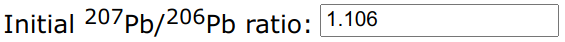
\includegraphics[width=\linewidth]{../figures/initialPb76.png}
  \end{minipage}
  \begin{minipage}[t]{.6\linewidth}
    If \texttt{nominal} has been selected, and the data are of formats
    1--3, a new text box appears with the
    \textsuperscript{207}Pb/\textsuperscript{206}Pb ratio of the
    common Pb.
  \end{minipage}

\begin{script}
settings('iratio','Pb207Pb206',1.106)
radialplot(UPb1,common.Pb=1)
\end{script}

  \noindent\begin{minipage}[t]{.4\linewidth}
  \strut\vspace*{-\baselineskip}\newline
  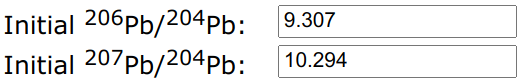
\includegraphics[width=\linewidth]{../figures/initialPb764.png}
  \end{minipage}
  \begin{minipage}[t]{.6\linewidth}
    For U--Pb data formats 4--6, the nominal common Pb composition is specified
    as a pair of \textsuperscript{206}Pb/\textsuperscript{204}Pb and 
    \textsuperscript{207}Pb/\textsuperscript{204}Pb ratios.
  \end{minipage}

\begin{script}
settings('iratio','Pb206Pb204',9.307)
settings('iratio','Pb207Pb204',10.294)
weightedmean(UPb2,common.Pb=1)
\end{script}

  \noindent\begin{minipage}[t]{.4\linewidth}
  \strut\vspace*{-\baselineskip}\newline
  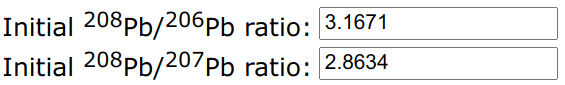
\includegraphics[width=\linewidth]{../figures/initialPb876.png}
  \end{minipage}
  \begin{minipage}[t]{.6\linewidth}
    Finally, for U--Pb data formats 7 and 8, the nominal common Pb
    composition is specified as a pair of
    \textsuperscript{208}Pb/\textsuperscript{206}Pb and
    \textsuperscript{208}Pb/\textsuperscript{207}Pb ratios.
  \end{minipage}

\begin{script}
settings('iratio','Pb208Pb206',3.1671)
settings('iratio','Pb208Pb207',2.8634)
weightedmean(UPb3,common.Pb=1)
\end{script}

\item\noindent\begin{minipage}[t]{.4\linewidth}
  \strut\vspace*{-\baselineskip}\newline
  
\includegraphics[width=\linewidth]{../figures/isochroncommonpb.png}
  \end{minipage}
  \begin{minipage}[t]{.6\linewidth}
    Selecting the \texttt{isochron} option implements the common Pb
    correction algorithm of
    Section~\ref{sec:common-Pb}.\ref{it:isochroncommonpb}. In other
    words, it projects all the aliquots parallel to the isochron and
    onto the radiogenic dimension. It is important to reiterate that
    selecting this option does \textbf{not} return the isochron age!
  \end{minipage}
  
\begin{script}
kde(UPb2,common.Pb=2)
\end{script}
  
\item\noindent\begin{minipage}[t]{.4\linewidth}
  \strut\vspace*{-\baselineskip}\newline
  
\includegraphics[width=\linewidth]{../figures/staceykramerscommonpb.png}
  \end{minipage}
  \begin{minipage}[t]{.6\linewidth}
    Selecting the \texttt{Stacey-Kramers} option implements the common
    Pb correction algorithm of
    Section~\ref{sec:common-Pb}.\ref{it:separate-stacey-kramers}.
  \end{minipage}

\begin{script}
cad(UPb1,common.Pb=3)
\end{script}

\end{enumerate}

\item Initial disequilibrium can be activated by ticking the
  corresponding box in the GUI, or by calling the \texttt{diseq()}
  function from the CLI. The output of the latter function must be
  called from the \texttt{read.data()} function.

\noindent\begin{minipage}[t]{.6\linewidth}
  \strut\vspace*{-\baselineskip}\newline
  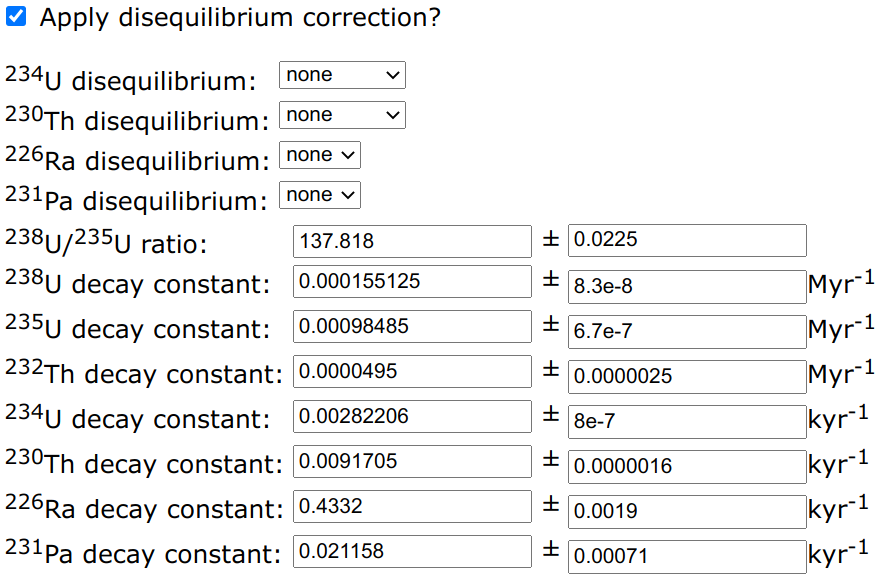
\includegraphics[width=\linewidth]{../figures/UPbDisequilibriumSettings.png}
  \end{minipage}
  \begin{minipage}[t]{.4\linewidth}
    Ticking the initial disequilibrium box reveals the decay constants
    of \textsuperscript{234}U, \textsuperscript{230}Th,
    \textsuperscript{226}Ra and \textsuperscript{231}Pa.  From the
    CLI, these parameters can be changed using the \texttt{settings()}
    function in exactly the same way as shown in
    Section~\ref{sec:general}.\ref{it:UPbLambdairatio}.
  \end{minipage}

\begin{enumerate}

\item There are two ways to specify the initial disequilibrium
  conditions for \textsuperscript{234}U and \textsuperscript{230}Th:
  
\noindent\begin{minipage}[t]{.6\linewidth}
  \strut\vspace*{-\baselineskip}\newline
  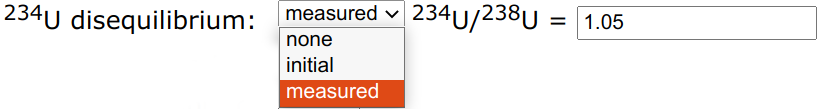
\includegraphics[width=\linewidth]{../figures/U234-disequilibrium.png}
  \end{minipage}
  \begin{minipage}[t]{.4\linewidth}
If the sample is young enough that secular equilibrium has not yet
been re-established, then any measured remanent disequilibrium can be
specified here.
  \end{minipage}

\noindent CLI example:
\begin{script}
d <- diseq(U48=list(x=1.05,option=2))
UPb <- read.data('diseq.csv',method='U-Pb',format=2,d=d)
concordia(UPb,type=2)
\end{script}

\item For the shortest lived isotopes \textsuperscript{226}Ra and
  \textsuperscript{231}Pa, only one option is available:
  
\noindent\begin{minipage}[t]{.6\linewidth}
  \strut\vspace*{-\baselineskip}\newline
  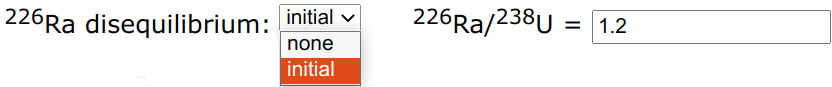
\includegraphics[width=\linewidth]{../figures/Ra226-disequilibrium.png}
\end{minipage}
\begin{minipage}[t]{.4\linewidth}
It is generally not possible to measure the remanent disequilibrium
for these isotopes, so the only option is to specify the hypothesised
initial activity ratio.
\end{minipage}

\noindent CLI example:
\begin{script}
d <- diseq(RaU=list(x=1.2,option=1))
UPb <- read.data('diseq.csv',method='U-Pb',format=2,d=d)
concordia(UPb,type=2)
\end{script}

\item Finally, for U--Pb data of formats 7 and 8 (which include the
  \texttt{232}Th/\textsuperscript{238}U ratio of the mineral), there
  is a fourth way to specify the initial
  \textsuperscript{230}Th/\textsuperscript{238}U activity ratio, by
  supplying the measured Th/U-ratio of the magma, determined by
  geochemical analysis of the whole rock or volcanic glass:

\noindent\begin{minipage}[t]{.6\linewidth}
    \strut\vspace*{-\baselineskip}\newline
    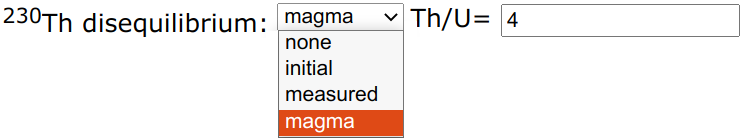
\includegraphics[width=\linewidth]{../figures/Th230-disequilibrium.png}
  \end{minipage}
  \begin{minipage}[t]{.4\linewidth}
    \texttt{IsoplotR} combines this measured ratio with the
    \textsuperscript{232}Th/\textsuperscript{238}U-ratio of the
    minerals to compute the Th/U fractionation factor.
  \end{minipage}

\noindent CLI example:
\begin{script}
d <- diseq(ThU=list(x=3,option=3))
UPb <- read.data('diseq.csv',method='U-Pb',format=8,d=d)
radialplot(UPb)
\end{script}

\end{enumerate}

The different disequilibrium settings can be combined in the GUI, and
from the command line using the \texttt{diseq} function:

\begin{script}
d <- diseq(U48=list(x=1.05,option=1),ThU=list(x=3,option=3),
           RaU=list(x=1.2,option=2),PaU=list(x=3,option=1))
UPb <- read.data('diseq.csv',method='U-Pb',format=2,d=d)
concordia(UPb,type=2)
\end{script}

\end{enumerate}

\section{concordia} \label{sec:concordia-R}

\noindent\begin{minipage}[t]{.3\linewidth}
  \strut\vspace*{-\baselineskip}\newline
  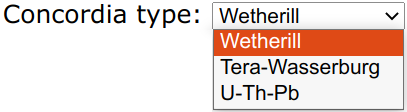
\includegraphics[width=\linewidth]{../figures/ConcordiaMenu.png}
\end{minipage}
\begin{minipage}[t]{.7\linewidth}
  \texttt{IsoplotR} offers three types of concordia diagrams. The
  U--Th--Pb diagram is only available for U--Pb data formats 7 and 8.
\end{minipage}

\begin{script}
concordia(UPb1,type=1) # Wetherill
concordia(UPb1,type=2) # Tera-Wasserburg
concordia(UPb3,type=3) # U-Th-Pb
\end{script}

\begin{enumerate}

\item The limits of the concordia diagram can be specified in two
  ways:

  \noindent\begin{minipage}[t]{.4\linewidth}
  \strut\vspace*{-\baselineskip}\newline
  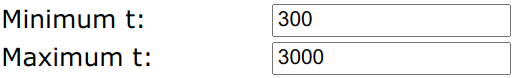
\includegraphics[width=\linewidth]{../figures/Concordiatlim.png}
\end{minipage}
\begin{minipage}[t]{.6\linewidth}
  The first option is to specify the minimum and maximum age of the
  concordia line.
\end{minipage}

\begin{script}
# Wetherill diagram from 300 to 3000 Ma:
concordia(UPb1,tlim=c(300,3000)) 
\end{script}

\noindent\begin{minipage}[t]{.4\linewidth}
  \strut\vspace*{-\baselineskip}\newline
  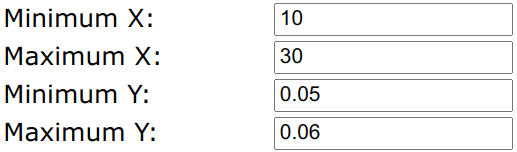
\includegraphics[width=\linewidth]{../figures/ConcordiaXYlim.png}
\end{minipage}
\begin{minipage}[t]{.6\linewidth}
  Alternatively, the limits of the concordia diagram can also be
  specified by the minimum and maximum extent of the horizontal and
  vertical axis.
\end{minipage}

\begin{script}
# Tera-Wasserburg diagram with U238/Pb206 limits from 10 to 30
# and Pb207/Pb206 limits from 0.05 to 0.06:
concordia(UPb1,type=2,xlim=c(10,30),ylim=c(0.05,0.06))
\end{script}

\item By default, \texttt{IsoplotR} plots error ellipses and
  calculates confidence intervals at a 95\% confidence level.

  \noindent\begin{minipage}[t]{.4\linewidth}
  \strut\vspace*{-\baselineskip}\newline
  
\includegraphics[width=\linewidth]{../figures/ConcordiaAlpha.png}
\end{minipage}
\begin{minipage}[t]{.6\linewidth}
To plot the data as `2 sigma' ellipses, this can be changed to
$\alpha=0.14$ here, which covers 86\% of the area under a bivariate
normal distribution:
\end{minipage}

\begin{console}
concordia(UPb1,alpha=0.14)
\end{console}

\item When an extra variable is entered in the optional \texttt{(C)}
  column of the input table, this can be used as a colour scale (see
  Section~\ref{sec:GUI}).

  \noindent\begin{minipage}[t]{.4\linewidth}
  \strut\vspace*{-\baselineskip}\newline
  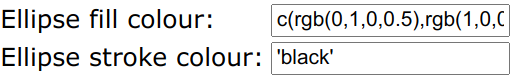
\includegraphics[width=\linewidth]{../figures/ConcordiaColours.png}
\end{minipage}
\begin{minipage}[t]{.6\linewidth}
  The corresponding fill and stroke colours can be specified by
  entering \texttt{R} code in the text box of the GUI.\\
\end{minipage}

\noindent To illustrate the different possibilities, let us consider a
U--Pb dataset of format~7 or 8 and use the Th/U ratios to build a
colour scale:
\begin{console}
ThU <- UPb3$x$Th232U238
\end{console}

\noindent Specify the fill colours by name:
\begin{console}
concordia(UPb3,levels=ThU,ellipse.fill=c('blue','red'))
\end{console}

\noindent Using red-green-blue-transparency (rgb-alpha) specifiers:
\begin{console}
concordia(UPb3,levels=ThU,ellipse.fill=c(rbg(1,0,0,0.5),rgb(0,1,0,0.5)))
\end{console}

\noindent Specifying the stroke colours as a colour palette with 80\% opacity
and using a uniform white colour for the fill colour:
\begin{script}
concordia(UPb3,levels=ThU,ellipse.fill='white',
          ellipse.stroke=heat.colors(n=10,alpha=0.8))
\end{script}

\noindent Leaving the error ellipses empty but using a reversed colour palette
for the stroke colour:
\begin{console}
concordia(UPb3,levels=ThU,ellipse.fill=NA,ellipse.stroke=rev(rainbow(n=10)))
\end{console}

\noindent\begin{minipage}[t]{.4\linewidth}
\strut\vspace*{-\baselineskip}\newline

\includegraphics[width=\linewidth]{../figures/UPbColourLabel.png}
\end{minipage}
\begin{minipage}[t]{.6\linewidth}
  Specifying colour levels adds a colour bar to the concordia diagram,
  which can be labelled for clarity.
\end{minipage}

\begin{console}
concordia(UPb3,levels=ThU,clabel='Th/U')
\end{console}

\item \texttt{IsoplotR} automatically chooses a `pretty' sequence of
  age ticks for the concordia line.

  \noindent\begin{minipage}[t]{.4\linewidth}
  \strut\vspace*{-\baselineskip}\newline
  
\includegraphics[width=\linewidth]{../figures/Concordiatticks.png}
\end{minipage}
\begin{minipage}[t]{.6\linewidth}
  These default values can be overruled by a comma separated list of
  numerical values (in Myr).
\end{minipage}

\begin{console}
concordia(UPb1,ticks=c(230,240,250))
\end{console}

Alternatively, the \texttt{ticks} argument can also be used to simply
specify the number of ticks:

\begin{console}
concordia(UPb1,ticks=10)
\end{console}

\item Labelling the error ellipses can be useful to identify outliers
  or otherwise noteworthy aliquots.

  \noindent\begin{minipage}[t]{.3\linewidth}
  \strut\vspace*{-\baselineskip}\newline
  
\includegraphics[width=\linewidth]{../figures/concordiashownumbers.png}
\end{minipage}
\begin{minipage}[t]{.7\linewidth}
  Ticking the box labels the ellipses with the row numbers of the
  input data.
\end{minipage}

\begin{console}
concordia(UPb1,show.numbers=TRUE)
\end{console}

\item The font size of the sample numbers, axis labels, and any legend
  can be adjusted with a multiplier.

\noindent\begin{minipage}[t]{.3\linewidth}
\strut\vspace*{-\baselineskip}\newline

\includegraphics[width=\linewidth]{../figures/concordiacex.png}
\end{minipage}
\begin{minipage}[t]{.7\linewidth}
Values greater than 1 increase the font size, values less than 1
reduce it.  
\end{minipage}

At the CLI, the font size is controlled by the environment variable
\texttt{cex}, which can be changed with the \texttt{par()} function:

\begin{script}
oldpar <- par(cex=1.2)
concordia(UPb1,show.numbers=TRUE)
par(oldpar) # restore the old cex value
\end{script}

\item Besides a data visualisation device, the concordia diagram can
  also be used as a vehicle for various numerical calculations:

\noindent\begin{minipage}[t]{.3\linewidth}
  \strut\vspace*{-\baselineskip}\newline
  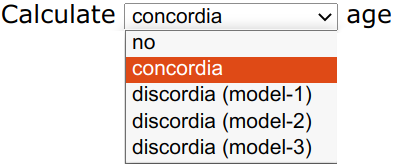
\includegraphics[width=\linewidth]{../figures/ConcordiaShowAge.png}
\end{minipage}
\begin{minipage}[t]{.7\linewidth}
  Selecting the \texttt{concordia} option adds a white ellipse with
  the concordia composition to the plot, as well as a legend with the
  concordia age, confidence intervals, MSWD and p-values.
\end{minipage}

Compute the concordia age of the first 9 aliquots. Show the
10\textsuperscript{th} aliquot but do not use it for the calculation:

\begin{console}
concordia(UPb1,show.age=1,omit=10)
\end{console}

\item Decay constant uncertainties can be visualised as a thicker
  concordia line, and propagated into any derived numerical values.

\noindent\begin{minipage}[t]{.35\linewidth}
\strut\vspace*{-\baselineskip}\newline

\includegraphics[width=\linewidth]{../figures/concordiaexterr.png}
\end{minipage}
\begin{minipage}[t]{.65\linewidth}
  Ticking the box adds the decay constant (and
  \textsuperscript{238}U/\textsuperscript{235}U ratio) uncertainty
  after the concordia composition has been calculated.
\end{minipage}

The following code snippet does not only omit the
10\textsuperscript{th} aliquot from the calculation, but also removes
it from the plot altogether. The external uncertainties are added by
the optional \texttt{exterr} argument:

\begin{console}
concordia(UPb1,show.age=1,hide=10,exterr=TRUE)
\end{console}


\end{enumerate}

\section{isochrons} \label{sec:UPb-isochron-R}

\printbibliography[heading=subbibliography]

\end{refsection}
